\chapter{Исследовательская часть}

В данной части будет проводено исследование разработанных алгоритмов компьютерной графики для использования их с применением аппаратных возможностей микроконтроллера. 

Целью исследования является определение зависимости времени выполнения классического и модифицированного алгоритмов Варнока от количества визуализируемых полигонов на сцене, а также сравнение данных алгоритмов. Замеры времени проводятся для количества полигонов, изменяющегося от 50 до 500 с шагом измерения в 50 полигонов. 

\section{Средства реализации}
При проведении исследования используется микроконтроллер RP2040~\cite{rp2040} в плате Raspberry Pi Pico. Для отображения итогового изображения используются два экрана с разрешением 240x240 пикселов, подключенные по одной шине SPI. 

Характеристики микроконтроллера RP2040:
\begin{itemize}
    \item 32-битный процессор ARM Cortex-M0+~\cite{cortex-m0};
    \item тактовая частота процессора -- 133 МГц;
    \item объем оперативной памяти -- 264 Кб;
    \item объем постоянной памяти -- 2 Мб;
    \item частота шины SPI -- 40 МГц;
    \item наличие встроенного контроллера DMA~\cite{dma}. 
\end{itemize}

Для замера времени работы реализованных алгоритмов используется системый системный таймер SysTick~\cite{systick}, который является частью процессоров семейства Cortex-M. 

\section{Результаты исследования}
В таблице \ref{tbl:time} приведены результаты замеров времени для двух реализаций алгоритма Варнока удаление невидимых граней.

\begin{table}[H]
    \caption{\label{tbl:time}Замеры времени сравнения алгоритмов Варнока}
	\resizebox{\textwidth}{!}{
	\def\arraystretch{1}
    \begin{tabular}{|c|c|c|}
    \hline
    Кол-во полигонов, шт &
      \begin{tabular}[c]{@{}c@{}}Модифицированный \\ алгоритм Варнока, мс\end{tabular} &
      \begin{tabular}[c]{@{}c@{}}Классический \\ алгоритм Варнока, мс\end{tabular} \\ \hline
    50  & 1452  & 2032  \\ \hline
    100 & 3132  & 4698  \\ \hline
    150 & 5076  & 7360  \\ \hline
    200 & 6349  & 8903  \\ \hline
    250 & 9071  & 12699 \\ \hline
    300 & 10865 & 14124 \\ \hline
    350 & 12168 & 18435 \\ \hline
    400 & 15323 & 22984 \\ \hline
    450 & 17342 & 23744 \\ \hline
    500 & 19891 & 29836 \\ \hline
    \end{tabular}
    }
\end{table}

На рисунке \ref{img:plot} представлен график зависимости времени работы двух алгоритмов Варнока в зависимости от заданного количества полигонов.

\begin{figure}[H]
	\centering
	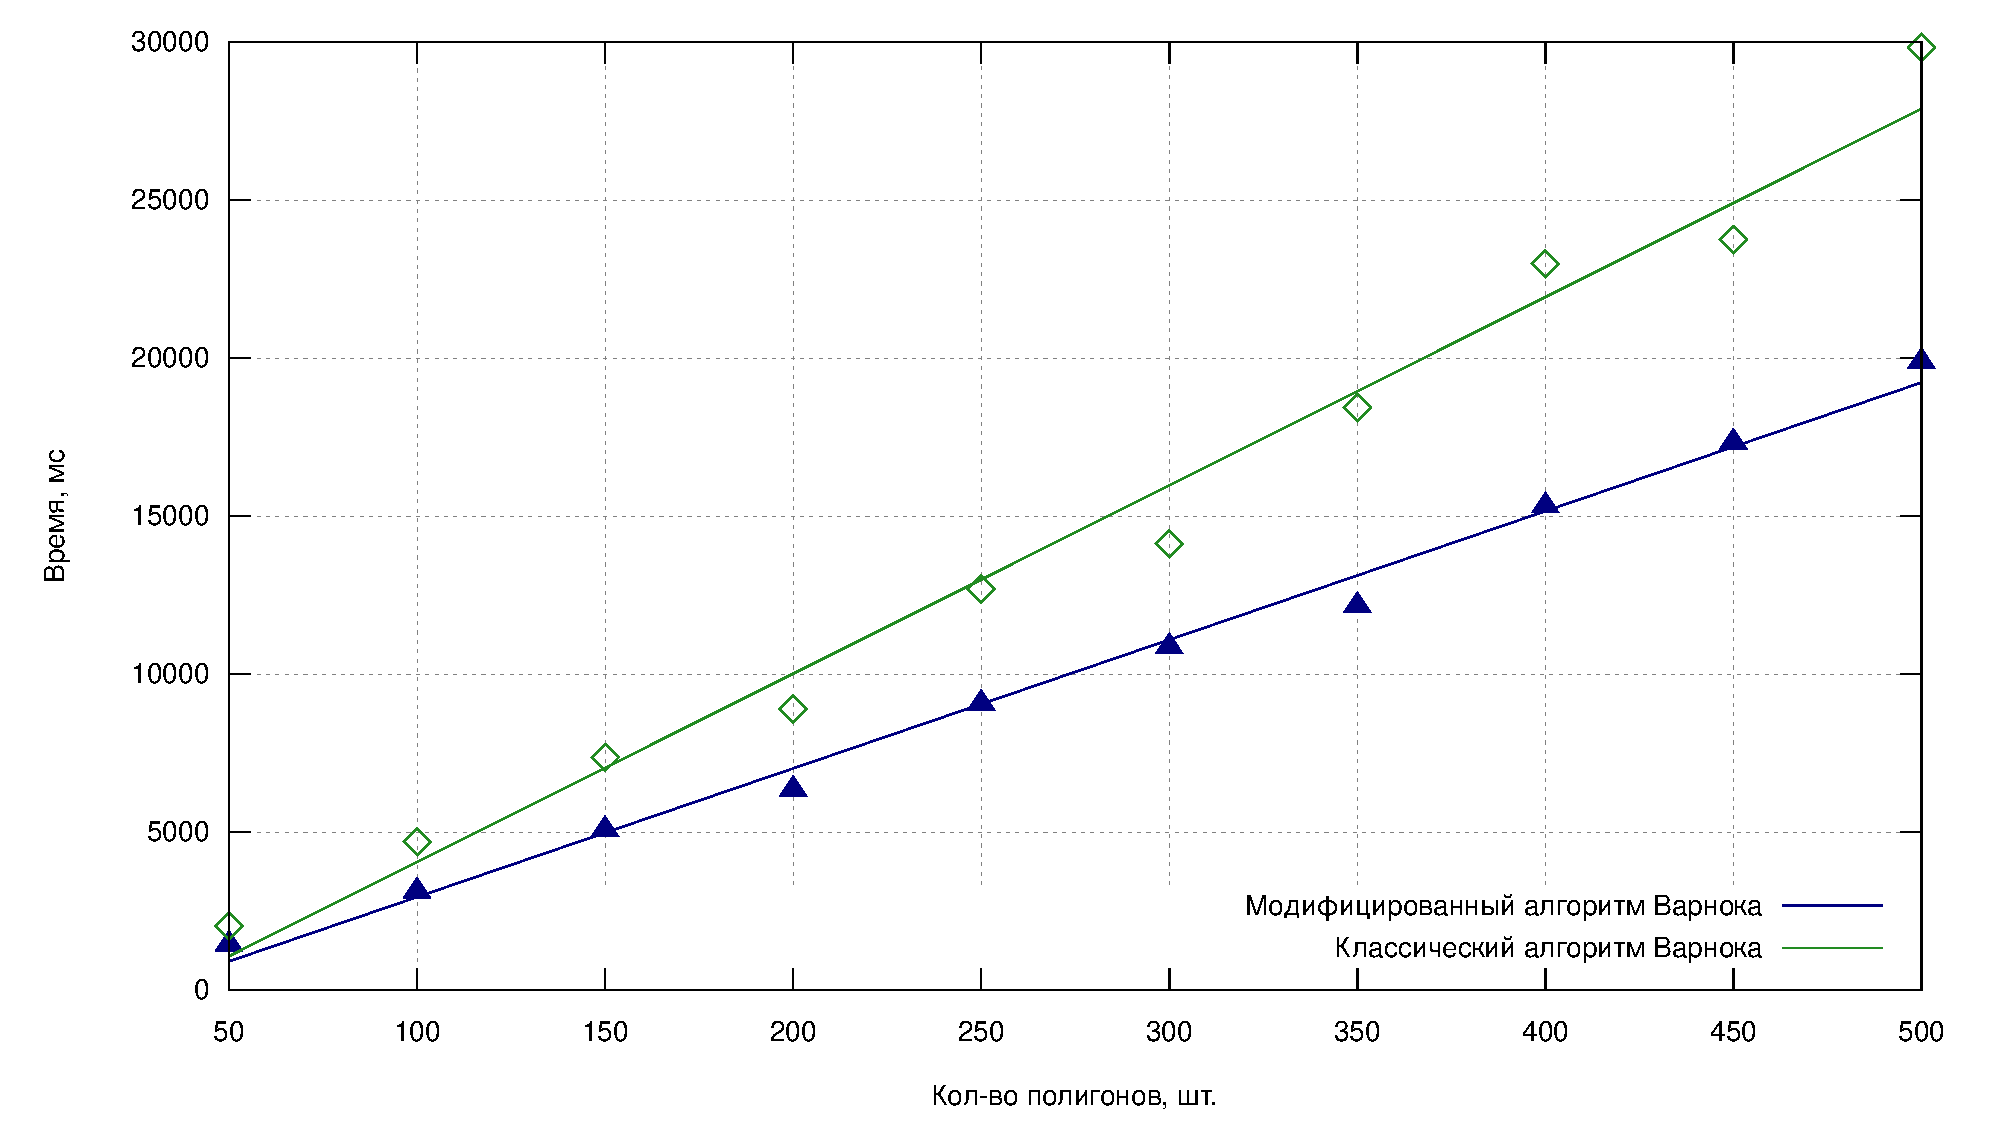
\includegraphics[height=0.35\textheight]{inc/img/plot.pdf}
	\caption{Сравнение классического и модифицированного алгоритмов Варнока}
	\label{img:plot}
\end{figure}

\section{Вывод из исследовательской части}
В результате исследования можно заметить, что модифицированный алгоритм Варнока превосходит классическую реализацию алгоритма по эффективности. Таким образом, за счет использования аппаратных особенностей микроконтроллера удалось достичь меньшего времени визуализации сцены. Прямой доступ к памяти обеспечивает более эффективный доступ к периферии, при этом нагрузка на процессор не увеличивается.
